% Format teze zasnovan je na paketu memoir
% http://tug.ctan.org/macros/latex/contrib/memoir/memman.pdf ili
% http://texdoc.net/texmf-dist/doc/latex/memoir/memman.pdf
% 
% Prilikom zadavanja klase memoir, navedenim opcijama se podešava 
% veličina slova (12pt) i jednostrano štampanje (oneside).
% Ove parametre možete menjati samo ako pravite nezvanične verzije
% mastera za privatnu upotrebu (na primer, u b5 varijanti ima smisla 
% smanjiti 
\documentclass[12pt,oneside]{memoir} 
% Paket koji definiše sve specifičnosti master rada Matematičkog fakulteta
\usepackage[latinica]{matfmaster} 


\usepackage{listings}


\lstdefinestyle{customc}{
  belowcaptionskip=1\baselineskip,
  breaklines=true,
  frame=L,
  xleftmargin=\parindent,
  language=C++,
  showstringspaces=false,
  basicstyle=\footnotesize\ttfamily,
  keywordstyle=\bfseries\color{green!40!black},
  commentstyle=\itshape\color{purple!40!black},
  identifierstyle=\color{blue},
  stringstyle=\color{orange},
  numbers=left,
  numberstyle=\tiny,
}

\lstdefinestyle{customasm}{
  belowcaptionskip=1\baselineskip,
  frame=L,
  xleftmargin=\parindent,
  language=[x86masm]Assembler,
  basicstyle=\footnotesize\ttfamily,
  commentstyle=\itshape\color{purple!40!black},
}


\lstdefinestyle{BashInputStyle}{
  language=bash,
  belowcaptionskip=1\baselineskip,
  basicstyle=\small\sffamily,
  numbers=left,
  numberstyle=\tiny,
  numbersep=3pt,
  frame=tb,
  columns=fullflexible,
  backgroundcolor=\color{yellow!20},
  linewidth=0.9\linewidth,
  xleftmargin=0.1\linewidth,
}

\lstdefinestyle{custombash}{
  belowcaptionskip=1\baselineskip,
  frame=L,
  xleftmargin=\parindent,
  language=[x86masm]Assembler,
  basicstyle=\footnotesize\ttfamily,
  commentstyle=\itshape\color{purple!40!black},
  backgroundcolor=\color{yellow!20},
  numbers=left,
  numberstyle=\tiny,
}
% \lstset{%
% language=C++,
% frame=XL,
% numbers=left,
% numberstyle=\footnotesize,
% tabsize=2,
% keepspaces=true,
% columns=fullflexible,
% stringstyle=\color{red}\ttfamily,
% basicstyle=\fontsize{11}{10}\ttfamily,
% keywordstyle=\color{blue},
%   belowskip=1em,
%   aboveskip=1em
% }

% \lstset{language=C++,
%                 basicstyle=\ttfamily,
%                 keywordstyle=\color{blue}\ttfamily,
%                 stringstyle=\color{red}\ttfamily,
%                 commentstyle=\color{green}\ttfamily,
%                 morecomment=[l][\color{magenta}]{\#}
% }

% \usepackage[serbian]{babel}%
% Podrazumevano pismo je ćirilica.
%   Ako koristite pdflatex, a ne xetex, sav latinički tekst na srpskom jeziku
%   treba biti okružen sa \lat{...} ili \begin{latinica}...\end{latinica}.
%
% Opicija [latinica]:
%   ako želite da pišete latiniciom, dodajte opciju "latinica" tj.
%   prethodni paket uključite pomoću: \usepackage[latinica]{matfmaster}.
%   Ako koristite pdflatex, a ne xetex, sav ćirilički tekst treba biti
%   okružen sa \cir{...} ili \begin{cirilica}...\end{cirilica}.
%
% Opcija [biblatex]:
%   ako želite da koristite reference na više jezika i umesto paketa
%   bibtex da koristite BibLaTeX/Biber, dodajte opciju "biblatex" tj.
%   prethodni paket uključite pomoću: \usepackage[biblatex]{matfmaster}
%
% Opcija [b5paper]:
%   ako želite da napravite verziju teze u manjem (b5) formatu, navedite
%   opciju "b5paper", tj. prethodni paket uključite pomoću: 
%   \usepackage[b5paper]{matfmaster}. Tada ima smisla razmisliti o promeni
%   veličine slova (izmenom opcije 12pt na 11pt u \documentclass{memoir}).
%
% Naravno, opcije je moguće kombinovati.
% Npr. \usepackage[b5paper,biblatex]{matfmaster}

% Pomoćni paket koji generiše nasumičan tekst u kojem se javljaju sva slova
% azbuke (nema potrebe koristiti ovo u pravim disertacijama)
% \usepackage[latinica]{pangrami}

% Datoteka sa literaturom u BibTex tj. BibLaTeX/Biber formatu
\bib{MasterRadOgnjenPlavsic}

% Ime kandidata na srpskom jeziku (u odabranom pismu)
\autor{Ognjen Ž. Plavšić}
% Naslov teze na srpskom jeziku (u odabranom pismu)
\naslov{Alat za stati\v{c}ku analizu i predlaganje izmena u C++ kodu}
% Godina u kojoj je teza predana komisiji
\godina{2022}
% Ime i afilijacija mentora (u odabranom pismu)
\mentor{dr Milena \textsc{Vujošević Janičić}, vanredni profesor\\ Univerzitet u Beogradu, Matematički fakultet}
% Ime i afilijacija prvog člana komisije (u odabranom pismu)
\komisijaA{dr Filip \textsc{Marić}, vanredni profesor\\ Univerzitet u Beogradu, Matematički fakultet}
% Ime i afilijacija drugog člana komisije (u odabranom pismu)
\komisijaB{dr Jelena \textsc{Graovac}, docent\\ Univerzitet u Beogradu, Matematički fakultet}
% Ime i afilijacija trećeg člana komisije (opciono)
% \komisijaC{}
% Ime i afilijacija četvrtog člana komisije (opciono)
% \komisijaD{}
% Datum odbrane (odkomentarisati narednu liniju i upisati datum odbrane ako je poznat)
% \datumodbrane{}

% Apstrakt na srpskom jeziku (u odabranom pismu)
\apstr{%
% \pangrami
}
\usepackage{tcolorbox}
% Ključne reči na srpskom jeziku (u odabranom pismu)
\kljucnereci{računarstvo, \textsc{autosar}, clang, llvm, c++}

\begin{document}
% ==============================================================================
% Uvodni deo teze
\frontmatter
% ==============================================================================
% Naslovna strana
\naslovna
% Strana sa podacima o mentoru i članovima komisije
\komisija
% Strana sa posvetom (u odabranom pismu)
\posveta{Porodici}
% Strana sa podacima o disertaciji na srpskom jeziku
\apstrakt
% Sadržaj teze
\tableofcontents*

% ==============================================================================
% Glavni deo teze
\mainmatter
% ==============================================================================

% ------------------------------------------------------------------------------
\chapter{Uvod}
% ------------------------------------------------------------------------------
% \pangrami

% \section{Primeri korišćenja klasičnih \LaTeX{} elemenata}
% % Primeri citiranja
% Još jedan citat \cite{GuSh:243}.
% % Primeri navodnika
% Isprobavamo navodnike: "Rekao je da mu se javimo sutra".
% % Primer referisanja na tabelu (koja se javlja kasnije)
% U tabeli \ref{tbl:rezultati} koja sledi prikazani su rezultati eksperimenta.
% % Primer kraćeg ćiriličkog teksta
% {\cir Ово је пример ћириличког текста који се јавља у латиничком документу.}
% U ovoj rečenici se javlja jedna reč na {\cir ћирилици}.
% % Primer korišćenja fusnota
% Iza ove rečenice sledi fusnota.\footnote{Ovo je fusnota.}

% % Primer dužeg ćirličkog teksta
% \begin{cirilica}
%   Ово је мало дужи блок текста исписан ћириличким писмом у оквиру
%   латиничког документа. Фијуче ветар у шибљу, леди пасаже и куће иза
%   њих и гунђа у оџацима.
% \end{cirilica}

% % Primer korišćenja tabele
% \begin{table}
% \centering
% \caption{Rezultati}
% \label{tbl:rezultati}
% \begin{tabular}{c>{\centering}p{2cm}c}
% \toprule
% 1 & 2 & 3\\\midrule
% 4 & 5 & 6\\\cmidrule(rl){1-2}
% 7 & 8 & 8\\
% \bottomrule
% \end{tabular}
% \end{table}

% % Primer korišćenja slike
% \begin{figure}[!ht]
%   \centering
%   \label{fig:grafikon}
%   \includegraphics[width=0.5\textwidth]{graph.png}
%   \caption{Grafikon}
% \end{figure}


% % Primer jednostavnije matematičke formule
% Evo i jedan primer matematičke formule: $e^{i\pi} + 1 = 0$. 
% % Primer referisanja na sliku
% Na slici \ref{fig:grafikon} prikazan je jedan grafikon.

% % primer kompleksnije matematičke formule
% $$
% \int_a^b f(x)\ \mathrm{d}x \ =_{def}\ \lim_{\max{\Delta x_k \rightarrow 0}} \sum_{k=1}^n f(x_k^*)\Delta x_k
% $$

% % primer referisanja na poglavlja i strane poglavlja
% Više detalja biće dato u glavi \ref{chp:razrada} na strani \pageref{chp:razrada}.

% % primer liste
% Možemo praviti i nabrajanja:
% \begin{enumerate}
% \item Analiza 1
% \item Linearna algebra
% \item Analitička geometrija
% \item Osnovi programiranja
% \end{enumerate}

% \pangrami

% ------------------------------------------------------------------------------




\chapter{Standard kodiranja \textsc{AUTOSAR} C++14}
\label{chp:autosar}

\textit{AUTomotive Open System ARchitecture (\textsc{AUTOSAR})} je međunarodna organizacija proizvođača vozila, dobavljača, pružaoca usluga i kompanija iz automobilske industrije i industrija elektronike, poluprovodnika i softvera \cite{\textsc{autosar}Website}. 
Cilj \textsc{autosar}a je da stvori i uspostavi otvorenu i standardizovanu softversku arhitekturu za automobilske elektronske upravljačke jedinice (\textit{eng. Electronic Control Units (ЕCU)}.
Radi ostvarenja pomenutih ciljeva \textsc{autosar} definiše, između ostalog, pravila kodiranja u programskom jeziku C++14 za sigurnosno kriti\v{c}ne sisteme. Glavni sektor primene standarda kodiranja \textsc{autosar} C++14 je automobilska industrija, međutim ovaj standard može biti primenjen
i na druge aplikacije za uređaje sa ugrađenim računarom (\textit{eng. embedded systems}). Ovaj standard predstavlja nadogradnju MISRA C++:2008 standarda \cite{AutosarGuidelines}.

\section{Programski jezik C++}

\textbf{C++} je programski jezik op\v{s}te namene koji pru\v{z}a direktan i efikasan model hardvera u kombinaciji sa strukturama za definisanje lakih (eng. \textit{lightweight}) apstrakcija \cite{TheC++ProgrammingLanguage}. Kreirao ga je Danski softverski in\v{z}enjer Bjarne Stroustrup kao ekstenziju programskog jezika C. U trenutku kreiranja, Osnovno pro\v{s}irenje u odnosu na programski jezik C bilo je mogu\'{c}nost kreiranja korisni\v{c}ki definisanih tipova, odnosno klasa. C++ pripada grupi objektno orijentisanih jezika. 

\subsection{Dizajn programskog jezika C++}

Osnovna ideja iza dizajna programskog jezika C++ jeste da zadr\v{z}i dizajn jezika C ali ga i pro\v{s}iri tako da jezik, odnosno njegova sintaksa, bude bliska problemu koji re\v{s}ava. Tako implementiranim programskim jezikom se koncepti re\v{s}enja problema mogu izraziti direktno i koncizno.
U svrhu toga, C++ pru\v{z}a:
\begin{itemize}
  \item {Direktna preslikavanja ugrađenih operacija i tipova na hardver kako bi obezbedio efikasno kori\v{s}\'{c}enje memorije i efikasne niske (eng. \textit{low-level}) operacije.}
  \item {Priu\v{s}tive (u smislu ra\v{c}unarskih resursa) i fleksibilne mehanizme apstrakcija za podr\v{s}ku korisni\v{c}ki definisanih tipova koji se mogu koristiti sa istom sintaksom, u istom obimu i sa istim performansama kao ugrađeni tipovi.}
\end{itemize}

Dizajn C++-a je fokusiran na tehnike programiranja koje se bave osnovnim pojmovima ra\v{c}unarstva kao \v{s}to su memorija, mutabilnost, apstrakcija, upravljanje ra\v{c}unarskim resursima, izra\v{z}avanje algoritama, rukovanje gre\v{s}kama i modularnost. Jezik je dizajniran sa ciljem da \v{s}to vi\v{s}e olak\v{s}a sistemsko programiranje, odnosno pisanje programa koji direktno koriste hardverske resurse i kod kojih su ovi resursi u velikoj meri ograni\v{c}eni \cite{TheC++ProgrammingLanguage}.


\subsection{Standard C++14}

Programski jezik C++ je standardizovan od strane ISO (\textit{International Standard Organization}) radne grupe poznate kao JTC1/SC22/WG21 \cite{ISOWebsite}. Do sada je objavljeno \v{s}est revizija C++ standarda i trenutno se radi na reviziji \textit{C++23}. 
\indent

Standard \textit{C++14} predstavlja pro\v{s}irenje standarda \textit{C++11} uglavnom manjim pobolj\v{s}anjima i ispravljanjem gre\v{s}aka iz standarda \textit{C++11} . Standard \textit{C++11} sa druge strane uveo je velike izmene u odnosu da prethodnu reviziju standarda, \textit{C++03}. 
Standardi \textit{C++11/14} uveli su ve\'{c}inu fundamentalnih koncepta onog \v{s}to se danas smatra modernim C++-om. Ovde pre svega spadaju desne reference, "move" semantika i savr\v{s}eno prosleđivanje, pametni pokaziva\v{c}i, lambda funkcije, dedukcija tipova ali i mnogi drugi koncepti.

\section{Klasifikacija pravila}
Standard \textsc{autosar} C++14 definiše 342 pravila od kojih je:
\begin{itemize}
  \item {154 prisvojeno bez modifikacija iz MISRA C++:2008 standarda.}
  \item {131 prisvojeno iz drugih C++ standarda}
  \item {57 pravila je zasnovano na istraživanju, literaturi ili iz drugih resursa.}
\end{itemize}
Pravila su klasifikovana po nivou obaveze, mogućnosti ispitivanja saglasnosti koda sa pravilom korišćenjem algoritama
statičke analize i cilju korišćenja:

\subsection{Klasifikacija po nivou obaveze}
Klasifikacija po nivou obaveze deli pravila na obavezna i preporučena.
Obavezna pravila predstavljaju neophodne zahteve koje C++ k\^{o}d mora ispuniti kako bi bio u saglasnosti sa standardom. U slučaju kada ovo nije moguće,
formalna odstupanja moraju biti prijavljena.
Preporučena pravila predstavljaju zahteve koje C++ k\^{o}d treba da ispuni kad god je to mogu\'{c}e. Međutim, ovi zahtevi nisu obavezni. Pravila
sa ovim nivoom obaveze ne treba smatrati savetom ili sugestijom koja može biti ignorisana ve\'{c} ih treba pratiti uvek kada je to prakti\v{c}no izvodljivo. Za ova pravila ne moraju biti prijavljena formalna odstupanja.

\subsection{Klasifikacija po primenjivosti statičke analize}
Klasifikacija po primenjivosti statičke analize deli pravila na: 
\begin{enumerate}
  \item{automatizovana}
  \item{delimično automatizovana}
  \item{neautomatizovana}
\end{enumerate}
Automatizovana su ona pravila kod kojih se ispitivanje saglasnosti koda može u potpunosti automatizovati algoritmima statičke analize.
Kod delimično automatizovanih pravila se ispitivanje saglasnosti koda može samo delimilčno automatizovati, na primer, korišćenjem neke heuristike ili pokrivanjem određenog broja slučajeva upotrebe i služi kao dopuna pregleda koda.
Za neautomatizovana pravila statička analiza ne pruža razumnu podršku. Za ispitivanje saglasnosti koda sa neautomatizovanim pravilima koriste se druga sredstva, kao što je recimo pregled koda.

\indent
Većina pravila iz standarda \textsc{autosar} C++14 spadaju u automatizovana pravila. Alati za statičku analizu koda koji tvrde da podržavaju standard \textsc{autosar} C++14 moraju u potpunosti obezbediti podršku za sva automatizovana pravila i delimičnu podršku, u meri u kojoj je to moguće, za pravila koja se ne mogu u potpunosti ispitati algoritmima statičke analize \cite{AutosarGuidelines}.

\indent
Primenjivost statičke analize na proveru saglasnosti koda sa određenim pravilom u velikoj meri zasniva se na teorijskoj klasifikaciji problema
na odlučive i neodlučive probleme. Ukoliko se pravilo zasniva na neodlučivom problemu možemo sa sigurnošću reći da alati za statičku analizu nisu u mogućnosti da u potpunosti ispitaju saglasnost koda sa ovim pravilom. Pravilo će biti klasifikovano kao parcijalno automatizovano ili neautomatizovano ukoliko detektovanje kršenja pravila obuhvata određivanje vrednosti koju promenljiva sadrži u fazi izvr\v{s}avanja ili da li program doseže određeni deo programa.

Primer parcijalno automatizovanog pravila je: 

\begin{center}
% [title=My heading line]

\begin{tcolorbox}
 M5-8-1 (obvezno, implementaciono, parcijalno automatizovano) \\
Desni operand šift operacije treba biti manji za broj između nula i jedan
od bitske širine tipa levog operanda.

\end{tcolorbox}
\end{center}

  Pravilo nije moguće u potpunosti automatizovati jer je očigledno potrebno poznavati vrednost desnog operanda, što u opštem slučaju nije
  moguće precizno zaključiti. Primer ovakvog koda prikazan je na listingu 2.1. \\


\begin{lstlisting}[style=customc, caption={K\^{o}d koji ilustruje nemogućnost primene statičke analize},label={lst:label1},language=C++, captionpos=b]
#include <iostream>
#include <cstdint>
#include <cstdlib>

int main(){
  int8_t u8a = rand() % 100;
  u8a = (uint8_t) ( u8a << rand() % 10);
}
\end{lstlisting}
Međitim, ukoliko je desni operand konstanta ili promenljiva konstantnog izraza (klju\v{c}na re\v{c} \textit{constexpr}), vrlo je verovatno da će alat za statičku analizu biti u stanju
  da zaključi vrednost ove promenljive (s obzirom da su ove vrednosti poznate tokom kompilacije), a samim tim i ispitati saglasnost koda sa ovim pravilom.
  Primer ovakvog koda prikazan je na Listingu 2.2. \\

\begin{lstlisting}[style=customc, caption={K\^{o}d čija se ispravnost jednostavno može utvrditi statičkom analizom},label={lst:label2},language=C++, captionpos=b]
#include <iostream>
#include <cstdint>
#include <cstdlib>

int main(){
  int8_t u8a = rand() % 100;
  u8a = (uint8_t) ( u8a << 7);
}
\end{lstlisting}

  Napredniji alati za statičku analizu koji podržavaju simboličko izvršavanje programa (npr. \textit{Clang Static Analyzer} \cite{CSAWebsite}) mogu pokriti i znatno kompleksnije 
  slučajeve od slučaja prikazanog u Listingu 2.2.
  \\
  \indent 
  Ukoliko su pravila koja se odnose na implementaciju C++ projekta, odnosno na C++ konstrukte i semantiku programa, dovoljno kompleksna, može se desiti da u potpunosti nije moguće koristiti alate za statičku analizu. Ovo uglavnom znači da je broj slučajeva upotrebe koji algoritmi iz statičkih alata mogu pokriti, zanemarljiv. Međutim, određeni broj pravila koja su klasifikovana kao neautomatizovana odnose se na aspekte koda koji zavise od samog projekta
  u okviru kog je k\^{o}d napisan, stoga je nemoguće koristiti algoritme statičke analize.
  Primer ovakvog pravila je:

\begin{center}
\begin{tcolorbox}
Pravilo A1-4-2 (obvezno, implementaciono, neautomatizovano) \\
Kod treba da poštuje zadate granice metrika koda.
\end{tcolorbox}
\end{center}

  %  \\ \\
  % \textit{Pravilo A1-4-2 (obvezno, implementaciono, neautomatizovano)
  %         Sav k\^{o}d treba poštovati definisane granice metrika koda.} \\

  Kako bi se odredilo da li je k\^{o}d napisan u skladu sa ovim pravilom potrebno je poznavati koje metrike koda se koriste u okviru projekta i
  granice definisane za te metrike. S obzirom da je ovo specifično za sam projekat, mogu se koristiti interni alati za statičku analizu koda u kombinaciji
  sa manuelnim pregledom koda. 

\subsection{Klasifikacija pravila prema cilju primene}
Klasifikacija pravila prema cilju primene (slučaju upotrebe) deli pravila na:

\begin{enumerate}
  \item{implementaciona}
  \item{verifikaciona}
  \item{pravila za alate}
  \item{infrastrukturna}
\end{enumerate}

Implementaciona pravila se odnose na implementaciju projekta odnosno na k\^{o}d, arhitekturu i dizajn.
Primer implementacionog pravila:

\begin{center}
\begin{tcolorbox}
Pravilo A2-9-1 (obvezno, implementaciono, automatizovano) \\
Ime heder fajla mora biti identično imenu tipa deklarisanog u njemu ukoliko deklariše tip.
\end{tcolorbox}
\end{center}


Verifikaciona pravila odnose se na proces verifikacije koji uključuje pregled koda, analizu i testiranje.
Primer verifikacionog pravila:

\begin{center}
\begin{tcolorbox}
Pravilo A15-0-6 (obvezno, verifikaciono, neautomatizovano) \\
Analiza treba biti izvršena kako bi se detektovalo loše rukovanje izuzecima. Treba analizirati slede\'ce slučajeve lošeg rukovanja izuzecima: \\
(a) Najgore vreme izvršavanja ne postoji ili se ne može utvrditi, \\
(b) Stek nije korektno raspakovan, \\
(c) Izuzetak nije bačen, drugačiji izuzetak je bačen, aktivirana je pogre\v{s}na "catch" naredba, \\
(d) Memorija nije dostupna tokom rukovanja izuzecima.
\end{tcolorbox}
\end{center}

Pravila za alate odnose se na softverske alate kao što su pretprocesor, kompajler, linker i biblioteke kompajlera.
Infrastrukturna pravila odnose se na operativni sistem i hardver \cite{\textsc{autosar}Guidelines}.
Primer pravila za alate koje je ujedno i infrastrukturno pravilo:

\begin{center}
\begin{tcolorbox}
Pravilo A0-4-1 (obvezno, pravilo za infrastrukturu/alate, neautomatizovano) \\
Implementacija brojeva u pokretnom zarezu treba da bude u skladu sa standardom IEEE 754.
\end{tcolorbox}
\end{center}





\chapter{Kompajlerska infrastruktura LLVM}
\label{chp:llvm}

Kompajlerska infrastruktura LLVM predstavlja kolekciju modularnih i ponovo iskoristivih kompajlerskih tehnologija i alata.
Započet je 2000. godine kao instraživački projekat Krisa Latnera (\textit{eng. Chris Lattner}) i Vikrama Advea (\textit{eng. Vikram Adve}) na Univerzitetu Ilinois.

LLVM podržava kompilaciju različitih programskih programiskih jezika na mnoštvo različitih arhitektura hardvera. Jednostavnost dodavanja podrške kompilacije programskog jezika za hardversku arhitekturu omogućeno je fleksibilnim dizajnom kod kog je infrastruktura kompajlera ugrubo podeljena na 3 dela: prednji (eng. \textit{frontend}), srednji (eng. \textit{middle-end}) i zadnji (eng. \textit{backend}). 

\begin{enumerate}
  \item Prednji deo LLVM-a prevodi izvordni k\^od podr\v{z}anih jezika u LLVM međukod. U ovu fazu spadaju leksi\v{c}ka, sintaksna i semanti\v{c}ka analiza
  izvornog koda, kreiranje apstraktnog sintaksnog stabla (eng. \textit{abstract syntax tree} (AST)) i generisanje LLVM međukoda koriste\'{c}i informacije iz AST-a
  \item{Srednji deo kompajlera vr\v{s}i niz optimizacija nad instrukcijama LLVM međukoda (eng. \textit{intermediate representation (IR))}. LLVM međukod predstavlja apstrakciju asemblera koja je nezavnisna od arhitekture hardvera. LLVM međukod zasnovan je na stati\v{c}nom pojedina\v{c}nom dodeljivanju (eng \textit{Static Single Assignment} (SSA)), strogo je tipiziran, fleksibilan i omogu\'{c}ava jednostavnu reprezentaciju svih jezika visokog nivoa (eng. \textit{high-level languages}).}
  \item{Zadnji deo kompajlera vr\v{s}i ma\v{s}inski zavisne optimizacije koda i generi\v{s}e ma\v{s}inski k\^{o}d  za ciljnu arhitekturu.}
\end{enumerate}

% \usepackage{float}
\begin{figure}[!h]
\begin{center}
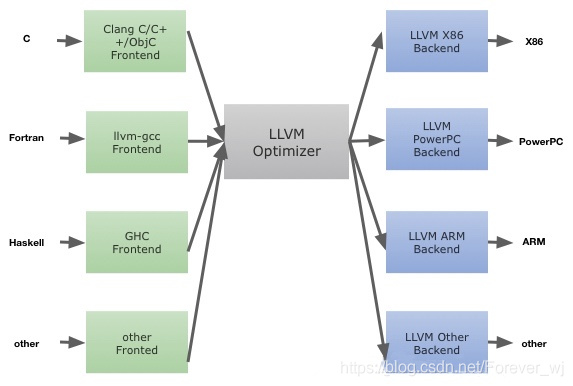
\includegraphics[scale=0.4]{llvmDesign.jpg}
\end{center}
\caption{Dizajn kompajlerske infrastrukture LLVM}
\label{fig:exploded}
\end{figure}

\section{Clang}

Clang projekat predstavlja prednji deo (\textit{eng. frontend}) LLVM kompajlerske infrastrukture za C familiju jezika (C, C++, Objective C/C++, OpenCL ...).
Pored optimizacija i efikasnog generisanja LLVM međukoda karakterističan je po ekspresivnosti dijagnostike odnosno kvalitetu poruka upozorenja i grešaka prijavljenih za izvorni kod. Dizajn Clang-a se sastoji od mnoštva biblioteka od kojih su najznačajnije za dizajn sledeće:

\begin{enumerate}
  \item{\textbf{Lekser i Pretprocesor} \\
       Implementiraju leksičku analizu i pretprocesiranje izvornog koda.
       Pretprocesor pru\v{z}a mogućnost uslovne kompilacije, uključivanja datoteka zaglavlja i proširenja makroa.
       Lekser kreira niz tokena od sintakse izvornog koda.}
  \item{\textbf{Parser} \\
        Kreira sintaksne strukture C++-a od niza tokena dobijenih leksičkom analizom.
        Clang-ov parser je implementiran kao parser rekurzivnog spuštanja (eng. \textit{recursive-descent parser}), odnosno analizira izvorni k\^{o}d  od vrha ka dnu nizom rekurzivnih funkcija \cite{LLVMCoreLibraries}.}
  \item{\textbf{AST biblioteka} \\
        Ova biblioteka implementira algoritme i strukture podataka koje parser koristi za izgradnju AST-a. Specifična je po strukturi čvorova koji podsećaju na izvorni C++ k\^{o}d  što je čini pogodnim za kreiranje alata za refaktorisanje koda i statičku analizu.}
  \item{\textbf{Sema} \\
        Vrši semantičku analizu programa tokom parsiranja i od semantički validnih konstrukta kreira AST. Usko je povezana sa parserom i AST bibliotekom.}
  \item{\textbf{Biblioteka za generisanje koda (eng. CodeGen Library)} \\
        Dobija AST kao ulaz i od njega generiše LLVM međukod.}

\end{enumerate}

\begin{figure}[!ht]
  \centering
  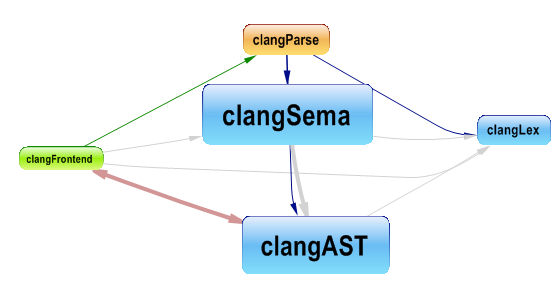
\includegraphics[width=1\textwidth]{ClangBiblioteke.png}
  \caption{Odnos osnovnih biblioteka Clang-a.}
  \label{fig:grafikon}
\end{figure}

\section{AST biblioteka}

U računarstvu, \textbf{apstraktno sintaksno stablo} (eng. abstract syntax tree (AST)), ili samo \textbf{sintaksno stablo}, je drvoidna reprezentacija apstraktne sintaktičke strukture izvornog koda napisanog u programskom jeziku. Svaki čvor stabla predstavlja konstrukt koji se pojavljuje u izvornom kodu.
Sintaksa je apstraktna u smislu da ne sadr\v{z}i svaki detalj koji se pojavljuje u sintaksi, ali sadr\v{z}i sve detalje neophodne za nedvosmislen prikaz izvornog koda.

Ekspresivnost Clang-ove dijagnostike i jednostavnost kreiranja mo\'{c}nih alata za stati\v{c}ku analizu u velikoj meri oslanja se na dizajn Clang-ove AST biblioteke. Struktura AST-a mo\v{z}e se jednostavno ispisati na standardni izlaz Clang-ovom \\ \texttt{-ast-dump} opcijom. Komanda na listingu \ref{lst:label3} ispisuje na standardni izlaz AST za k\^{o}d  iz fajla \texttt{hello.cpp} prikazanog na listingu \ref{lst:label4}. Slika \ref{fig:grafikon} predstavlja tekstualnu reprezentaciju AST-a ispisanu komandom iz listinga \ref{lst:label3}.
\\


\begin{lstlisting}[caption={Komanda za ispisivanje Clang-ovog AST-a},label=lst:label3,language=bash, captionpos=b]
$ clang -Xclang -ast-dump hello.c
\end{lstlisting}

\begin{lstlisting}[style=customc, caption={Kod \v{c}iji je AST prikazan na slici 4.1},label=lst:label4,language=C++, captionpos=b]
int main(){
  int a = 4;
  int b = 5;
  int result = a * b + 8;
}
\end{lstlisting}

% primer korišćenja slike
\begin{figure}[!ht]
  \centering
  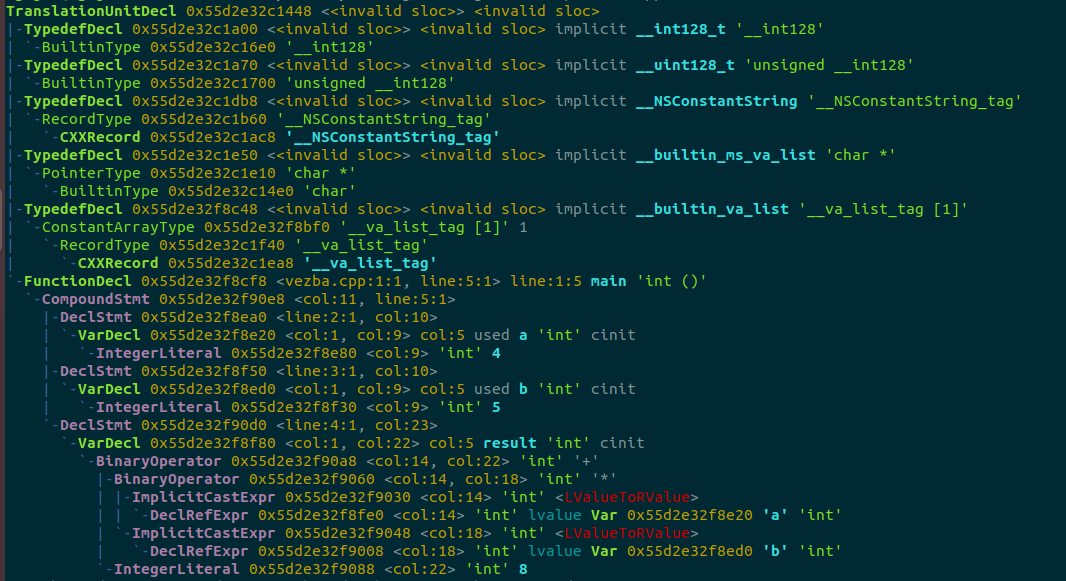
\includegraphics[width=1.0\textwidth]{ASTImage.png}
  \caption{Primer AST-a}
  \label{fig:grafikon}
\end{figure}

\v{C}vorovi od kojih je izgrađen AST predstavljaju apstrakciju sintaksnih struktura iz samog jezka.
Svi \v{c}vorovi Clang-ovog AST-a nasleđuju jednu od tri osnovne (bazne) klase:
\begin{itemize}
  \item \textit{\textbf{Decl}}
  \item \textit{\textbf{Stmt}}
  \item \textit{\textbf{Type}}
\end{itemize}
Ove klase redom opisuju deklaracije, naredbe i tipove iz C familije jezika.
Na primer \texttt{IfStmt} klasa opisuje \texttt{if} naredbe jezika i direktno nasleđuje \texttt{Stmt} klasu. Sa druge strane \texttt{FunctionDecl} i \texttt{VarDecl} klase, koje se koriste za opisivanje deklaracija i definicija funkcija i varijabli, ne nasleđuju dikertno klasu \texttt{Decl} ve\'{c} nasleđuju vi\v{s}e njenih podklasa.

\begin{itemize}
  \item \textit{\textbf{Klasa Type}} \\ Klasa \texttt{Type} bi\'{c}e posebno opisana s obizrom da igra va\v{z}nu ulogu u ekspresivnosti Clang-ove dijagnostike a samim tim i u kvalitetu alata za stati\v{c}ku analizu. Dizajn ove klase klju\v{c}an je za preciznost emitovanih poruka upozorenja i gre\v{s}aka u kodu. Na primer, upozorenja vezana za k\^{o}d  koji koristi tip \texttt{std::string}, ispisa\'{c}e ba\v{s} taj tip u svojim porukama umesto tipa koji \texttt{std::string} predefini\v{s}e, a to je \texttt{std::basic\_string<char, std:.. >}. Iza ove funkcionalnosti stoji ideja kanonskih tipova.
  
  \par
  Svaka instanca klase \texttt{Type} sadr\v{z}i pokaziva\v{c} na svoj kanonski tip. Za jednostavne tipove koji nisu definisani kori\v{s}\'{c}enjem \texttt{typedef} naredbe pokaziva\v{c} na kanonski tip \'{c}e zapravo pokazivati na sebe. Za tipove \v{c}ija struktura uklju\v{c}uje \texttt{typedef} naredbu kanonski pokaziva\v{c} pokaziva\'{c}e na strukturno ekvivalentan tip bez \texttt{typedef} naredbi.
  Na primer, kanonski tip tipa \texttt{int *} sa listinga \ref{lst:label5}  bi\'{c}e sam taj tip, dok \'{c}e kanonski tip za \texttt{foo *} biti \texttt{int *}.

\begin{lstlisting}[style=customc, caption={Demonstracija kanonskih tipova},label=lst:label5,language=C++, captionpos=b]
  int *a;
  typedef int foo;
  foo *b;
\end{lstlisting}
  Ovakvim dizajnom omogu\'{c}no je semanti\v{c}kim proverama da donose zaklju\v{c}ke direktno o pravom tipu ignori\v{s}u\'{c}i \texttt{typedef} naredbe kao i efikasno poređenje strukturne identi\v{c}nosti tipova.

  \par
  Klasa \texttt{Type} ne sadr\v{z}i informacije o kvalifikatorima tipova kao \v{s}to su \texttt{const}, \texttt{volatile}, \texttt{restrict} itd... Ove informacije enkapsulirane su u klasi \texttt{QualType} koja su\v{s}tinski predstavlja par pokaziva\v{c}a na tip (objekat klase \texttt{Type}) i bitova koji predstavljaju
  kvalifikatore. \v{C}uvanje kvalifikatora u vidu bitova omogu\'{c}uje veoma efikasno dohvatanje, dodavanje i brisanje kvalifikatora za tip. Postojanje ove klase smanjuje upotrebu hip memorije time \v{s}to se ne moraju kreirati duplikati tipova sa razli\v{c}itim kvalifikatorima. Na hipu se alocira jedan tip, a zatim 
  svi kvalifikovani tipovi pokazuju na alocirani tip na hipu sa dodatim kvalifikatorima \cite{CFEWebsite}.
\end{itemize}

\section{Biblioteke za obilazak AST-a}

Kompajlerska infrastruktura LLVM pru\v{z}a podr\v{s}ku za jednostavno kreiranje kvalitetnih alata za stati\v{c}ku analizu izvornog koda. Ovi alati
baziraju se na kori\v{s}\'{c}enju interfejsa ka Clang-ovom AST-u ili kori\v{s}\'{c}enjem stati\v{c}kog analizatora kompajlera Clang (eng. \textit{Clang Static Analyzer}) za potrebe simboli\v{c}kog izvr\v{s}avanja programa. Alati za stati\v{c}ku analizu mogu koristiti kombinaciju tehnika obilaska AST-a i simboli\v{c}kog izvr\v{s}avanja programa u zavisnosti od kompleksnosti analize koja je potrebna. Biblioteke za obilazak AST-a su jeftinije za kori\v{s}\'{c}enje po pitanju ra\v{c}unarskih resursa ali su ograni\v{c}ene informacijama dostupnim tokom kompilacije programa. Alati koji se implementiraju kao deo sistema za prevođenje programa omogu\'{c}avaju dodatnu optimizaciju procesa pronala\v{z}enja nepravilnih konstrukta direktnim proverama tokom kompilacije. Ovo se mo\v{z}e posti\'{c}i nadogradnjom osnovnih delova kompajlera kao \v{s}to su Lexer, Parser ili Sema. \\Osnovne biblioteke za obilazak AST-a u okviru kompajlera Clang su AST posetioci (eng. \textit{ASTVisitors}) i  AST upariva\v{c}i (eng. \textit{ASTMatchers}).



\newtheorem{primer}{Primer}[section]

\subsection{AST posetioci}
AST posetioci implementiraju mehanizam obilaska Clang-ovog AST stabla, odnosno pru\v{z}aju interfejs
za pose\'{c}ivanje svakog \v{c}vora u AST stablu.
Logika AST posetioca sadr\v{z}ana je u šablonskoj klasi \texttt{RecursiveASTVisitor<Derived>}.
Ovo je klasa koja posećuje svaki čvor Clang-ovog AST stabla obilaskom u dubinu.
AST posetioc je svaka potklasa klase \texttt{RecursiveASTVisitor<Derived>}.
Klasa \texttt{RecursiveASTVisitor<Derived>} obavlja tri odvojena zadatka:

\begin{enumerate}
\item Obilazi AST tj. posećuje svaki AST čvor.
\item Za dati čvor ide uz klasnu hijerarhiju počevši od dinamičkog tipa čvora do klase na vrhu hijerarhije (npr. \texttt{Stmt}, \texttt{Decl} ili \texttt{Type}).
\item Za datu kombinaciju (čvor, klasa), gde je klasa neka od baznih klasa dinamičkog tipa čvora, zove funkcije koje korisnik može predefinisati kako bi posetio čvor.
\end{enumerate}
Ova tri zadatka obavljaju tri grupe metoda, redom:
\begin{enumerate}
  \item \texttt{TraverseDecl(Decl *x)} obavlja zadatak 1. Ovo je ulazna tačka za obilazak AST-a sa korenom u čvoru x. Ovaj metod poziva metod \\ \texttt{TraverseFoo(Foo *x)}, gde je \texttt{Foo} dinamički tip od \texttt{*x}, koji poziva metod \texttt{WalkUpFromFoo(x)}, a zatim rekurzivno posećuje decu čvora \texttt{x}. \\ \texttt{TraverseStmt(Stmt *x)} i \texttt{TraverseType(QualType x)} rade na sličan način.
 
\item \texttt{WalkUpFromFoo(Foo *x)} izvršava zadatak 2. Ne pokušava odmah da poseti decu čvora \texttt{x}, umesto toga prvo zove \texttt{WalkUpFromBar(x)}, gde je \texttt{Bar} direktna nadklasa klase \texttt{Foo}, i tek onda zove \texttt{VisitFoo(x)}.
\item \texttt{VisitFoo(Foo *x)} izvršava zadatak 3.
\end{enumerate}
Ove tri grupe metoda slede naredni poredak: \texttt{Traverse > WalkUpFrom > Visit}. Metoda (npr. \texttt{Traverse}) može pozvati samo metode iz svoje grupe metoda ili iz grupe metoda direktno ispod nje (u smislu predstavljenog poretka). Metoda ne može pozvati metode iz grupe iznad \cite{visitors}.
Primer posetioca prikazan je na listingu \ref{lst:label6}:
\begin{lstlisting}[style=customc, caption={Primer posetioaca koji pose\'{c}uje sve strukture, unije i klase i ispisuje lokaciju onih koji se zovu n::m::C \cite{ASTToolTutorial}},label=lst:label6,language=C++, captionpos=b]
class FindNamedClassVisitor : public RecursiveASTVisitor<FindNamedClassVisitor> {
public:
  explicit FindNamedClassVisitor(ASTContext *Context)
    : Context(Context) {}

  bool VisitCXXRecordDecl(CXXRecordDecl *Declaration) {

    if (Declaration->getQualifiedNameAsString() == "n::m::C") {

      FullSourceLoc FullLocation = Context->getFullLoc(Declaration->getBeginLoc());

      if (FullLocation.isValid())
        llvm::outs() << "Found declaration at "
                     << FullLocation.getSpellingLineNumber() << ":"
                     << FullLocation.getSpellingColumnNumber() << "\n";
    }

    return true;
  }

private:
  ASTContext *Context;
};
\end{lstlisting}

\par
Da bi se izvršila neka analiza izvornog koda pomoću AST posetioca dovoljno je naslediti klasu 
 \texttt{RecursiveASTVisitor<Derived>} i predefinisati željene \texttt{Visit} metode u okviru nje. Ukoliko je \texttt{Visit} metodama pronađena konstrukcija izvornog koda koja se iz nekog razloga smatra nepravilnom, moze se prijaviti upozorenje.

\subsection{AST upariva\v{c}i}

Biblioteka AST uprariva\v{c}a (eng. \textit{LibASTMatcher}) pruža oblasno specifičan jezik (eng. domain specific language) za kreiranje predikata nad Clang-ovim AST stablom. Ovaj oblasno specifičan jezik je napisan i može se koristiti u C++-u omogućavajući korisnicima da u istom programu pristupe željenom delu stabla i da nad tim čvorovima koriste C++ interfejs za analiziranje raznih atributa, lokacija, i ostalih informacija dostupnih na AST nivou.
\\ Na primer, za kreiranje upariva\v{c}a koji uparuje sve deklaracije klasa ili unija u AST stablu neke jedinice prevođenja, može se koristiti poziv \texttt{recordDecl()}. Za sužavanje pretrage, na primer za nalaženje deklaracija svih klasa ili unija sa imenom \texttt{Foo}, treba iskoristiti \texttt{hasName} matcher: Poziv \texttt{recordDecl(hasName("Foo"))} vraća upariva\v{c} koji uparuje klase i unije sa imenom \texttt{"Foo"} u bilo kom prostoru imena (eng. \texttt{namespace}). Podrazumevano, upariva\v{c}i koji prihvataju više drugih upariva\v{c}a koriste implicitno \texttt{allOf()} metod koji \'{c}e upariti sve delove stabla na koje referi\v{s}u njegovi argumenti koji su takođe upariva\v{c}i. Ovo omogućava dalje sužavanje pretrage. Na primer za uparivanje klasa koje nasleđuju \texttt{"Bar"}, upariva\v{c} bi izgledao ovako: \texttt{recordDecl(hasName("Foo"), isDerivedFrom("Bar"))}.
\par

Uopšteno, strategija kreiranja upariva\v{c}a se svodi da sledeće korake:
\begin{enumerate}
\item Na\'{c}i baznu klasu u Clang-ovom AST-u koju je potrebno upariti.
 
\item Na\'{c}i u \texttt{AST Matcher Reference} dokumentu upariva\v{c} koji ili uparuje \v{z}eljeni čvor ili su\v{z}ava pretragu.
\item Kreirati spoljašnji izraz za uparivanje i proveriti da li radi o\v{c}ekivano.
\item Prona\'{c}i upariva\v{c}e koji bi mogli upariti neki unutrašnji čvor iz željenog dela stabla.
\item Ponavljati postupak dok uparivanje željenog dela stabla nije završeno.
\end{enumerate}

Izrazi za uparivanje (eng. \textit{match expressions}) omogu\'{c}uju uparivanje delova AST stabla. Nakon uparivanja, nad uparenim konstruktom uglavnom se vr\v{s}i određena analiza, na primer ispitivanje saglasnosti konstrukta sa pravilom standarda za pravilno pisanje C++ koda.
\par
Zbog toga, upariva\v{c}i koji uparuju specifi\v{c}ne čvorove AST stabla se mogu "vezati" (eng. \textit{binding}). Na primer, \texttt{recordDecl(hasName("MyClass")).bind("id")} će vezati upareni \texttt{recordDecl} čvor za string \texttt{id} kako bi se kasnije mogao koristiti u povratnom pozivu upariva\v{c}a (eng. match callback) \cite{matchers}. Na listingu \ref{lst:label7} prikazan je primer AST upariva\v{c}a.

\begin{lstlisting}[style=customc, caption={Primer upariv\v{c}a koji pronalazi sve klase koje nisu obeležene atributom \texttt{final} i čiji destruktor nije virtuelan, CallBack klase i poziva upariva\v{c}a}, label=lst:label7,language=C++, captionpos=b]
DeclarationMatcher NonFinalClassWithNonVirtualDestructor::makeMatcher() {
  return cxxRecordDecl(isClass(), unless(isFinal()),
                    anyOf(hasMethod(cxxDestructorDecl(isPublic(),
                    unless(isVirtual()))),
                    unless(hasMethod(cxxDestructorDecl()))))
                .bind("nonFinalClassWithNonVirtualDestructor");
}

void NonFinalClassWithNonVirtualDestructor::
    NonFinalClassWithNonVirtualDestructorCallBack::run(
        const MatchFinder::MatchResult &Result) {

  const BoundNodes &BN = Result.Nodes;
  
  if (const clang::CXXRecordDecl *CRD = BN.getNodeAs<clang::CXXRecordDecl>(
          "nonFinalClassWithNonVirtualDestructor"))
    reportWarning(
        SM.getDiagnostics(), CRD->getBeginLoc(),
        diag::warn_non_final_class_with_non_virtual_destructor);
}

void NonFinalClassWithNonVirtualDestructor::runMatcher(
    clang::ASTContext &AC) {
  MatchFinder NonFinalClassWithNonVirtualDestructor;
  NonFinalClassWithNonVirtualDestructor.addMatcher(makeMatcher(), &CB);
  NonFinalClassWithNonVirtualDestructor.matchAST(AC);
}
\end{lstlisting}

% \section{Clang-ov Statički Analizator}
% Clang-ov Statički Analizator je alat za traženje grešaka u programu. Analizirajući izvorni kod, ovaj alat pokušava da simulira izvršavanje delova programa bez njihovog prevođenja i prijavljuje greške koje bi se zapravo desile u toku izvršavanja (eng. run-time errors). Kako ponašanje izvršnih programa zavisi od spoljašnjih faktora kao što su ulazne vrednosti, slučajni brojevi i ostale stvari, mehanizam analizatora (eng. analyzer engine) dodeljuje vrednosti sa algebarskim simbolima, i izvršava simbolička izračunavanja koristeći ove simbole. Takođe otkriva uslove nad simboličkim vrednostima i postavlja ograničenja nad njima.
% \par Kao rezultat, Clang-ov Statički Analizator može da nađe greške koje se pojavljuju na retkim putanjama tokom izvršavanja programa. Ipak, analizator može naći samo greške koje je specifično programiran da nađe. Inače, kad naiđe na neki problem, analiza nastavlja dalje i ne prijavljuje nikakvu grešku. Za svaku grešku koju analizator nađe, kao što je na primer dereferenciranje null pokazivača, postoji poseban modul, \textbf{checker}, koji reaguje na te greške tokom analize.
% \par
% Dakle, jezgro analizatora je odgovorno za simboličko izvršavanje programa, a checker-i se prijavljuju za događaje za koje su zainteresovani, proveravaju razne pretpostavke nad simboličkim vrednostima, i prijavljuju upozorenja ukoliko se ove pretpostavke ne mogu postaviti na određenom putu.
% \subsection{Vrste analize koje pruža Clang-ov Statički Analizator}
% Prva odluka koju obično morate doneti kad pravite checker je da li vam je potrebna analiza puteva (eng. path-sensitive analysis) tj. simboličko izvršavanje programa. Analiza puteva je mnogo sporija od kompilacije. Većinu zahtevnih izračunavanja izvršava jezgro analizatora, dok su checker-i uglavnom prilično brzi.
% \par 
% O sintaksnoj analizi u okviru Clang-ovog Statičkog Analizatora ovde neće biti reči jer su AST checkeri zapravo jako slični AST vizitorima i po implementaciji i po mogućnostima koje pružaju.
% \par
% Druga vrsta analize je analiza zasnovana na analiziranju grafa kontrole toka (eng. control flow graph).
% \subsection{Analiza grafa kontrole toka}
%  Graf kontrole toka je grafovska reprezentacija svih puteva kojima se moze proći kroz program tokom njegovog izvršavanja. Ovaj graf se pravi odvojeno za svaku funkciju. Svaki čvor grafa kontrole toka predstavlja osnovni blok naredbi koje ne zadrže nikakvo grananje, pa se stoga izvršavaju sekvencijano. Svaki osnovni blok se završava završnom naredbom (eng. terminator statement), koja je granajuća naredba ili naredba \texttt{return}.
% \par 
% Pogledajmo naredni kod:
% \begin{lstlisting}[caption={},frame=single, label=simple]
% function() {
%   int a = 1;
%   int b = 2;

%   if (b == 2) {
%     ++b;
%   }
%   int c = 3;
%   int d = 4;

%   while (a < 5) {
%     ++a;
%   }
%   int e = 5;
%   int f = 6;
% }
% \end{lstlisting}
%  Graf kontrole toka koji odgovara prikazanom kodu prikazan je na slici \ref{fig:cfg}:
% \begin{figure}[h!]
% \begin{center}
% \includegraphics[scale=0.3]{GrafKontroleToka.png}
% \end{center}
% \caption{Grafička reprezentacija grafa kontrole toka}
% \label{fig:cfg}
% \end{figure}
% \par
% Analiza grafa kontrole toka je korisna za pravljenje sigurnih provera, za koje je nepotrebno proći kroz sve moguće puteve programa. Na primer, ukoliko želimo da osiguramo da je neki uslov uvek false, pa je onda odgovarajući k\^{o}d  "mrtav", morali bismo da dosegnemo sve definicije svih promenljivih koje se koriste u izrazu pomenutog uslova, tako da bi ovde najkorisnija bila analiza grafa kontrole toka.

% Međutim, pogledajmo naredni kod:
% \begin{lstlisting}[caption={},frame=single, label=simple]
%  void function(){
%   int y, z;
%   if (x == 0) y = 5;
%   if (!x) z = 6;
% }
% \end{lstlisting}
% Na osnovu analize grafa kontrole toka ne bismo mogli da utvrdimo da ukoliko se izvrši put koji dolazi do bloka tela prvog if-a, sigurno se neće izvršiti put koji dolazi do tela drugog if-a. Analizom grafa kontrole toka bismo morali da ispitamo sve četiri putanje, a zapravo nas interesuju samo dve. Ovo čini analizu dosta manje korisnom.
% \subsection{Analiza eksplodirajućeg grafa}
% Eksplodirajući graf Clang-ovog Statičkog Analizatora je osnovna struktura podataka za analizu puteva koje izvršava jezgro statičkog analizatora. Jezgro pokušava da interpretira k\^{o}d  i pravi različite putanje čak i ako te putanje uključuju iste osnovne blokove grafa kontrole toka. Eksplodirajući graf se sadrži od svih puteva kroz graf kontrole toka koji se istražuju od strane jezgra analizatora, i nosi informacije o stanju programa na svakom putu i u svakoj naredbi. Čvorovi grafa, eksplodirajući čvorovi, su parovi koji se sastoje od stanja programa i lokacije u programu koji se trenutno analizira.
% \par
% Eksplodirajući graf za prethodni k\^{o}d  prikazan je na slici \ref{fig:exploded}:
% \begin{figure}[h!]
% \begin{center}
% \includegraphics[scale=0.2]{exploded_graph.png}
% \end{center}
% \caption{Grafička reprezentacija eksplodirajućeg grafa}
% \label{fig:exploded}
% \end{figure}
% \par
% Pogledajmo kako analiza puteva radi na ovom primeru. Analizator počinje da simulira prvu operaciju, poređenje vrednosti promenljive x sa nulom. Pošto je \texttt{x} nepoznata u ovom trenutku u analizi, ova vrednost će biti reprezentovana simbolom \texttt{reg<x>}.
% \\ kada je ovo poređenje simulirano, dostižemo završnu naredbu u grafu kontrole toka, if- naredbu. U zavisnosti od uslova, analizator razvija dva nova puta, jedan u kom je vrednost promenljive x jednaka nuli, i drugi u kom je različita od nule. Na osnovu toga prave se ograničenja nad simbolom \texttt{reg<x>}, u prvom slučaju će ograničenje biti 0, dok će u drugom ograničenje biti unija intervala \texttt{[-21417483648, -1]} i \texttt{ [1, 21417483647]}. U sličnom maniru se dalje nastavlja analiza \cite{static_analyzer}.

\section{Interfejsi za akcije nad prednjim delom kompajlera}

Akcije nad prednjim delom kompajlera predstavljaju analizu i upotrebu rezultata i informacija koje pru\v{z}a prednji deo kompajlera. Ove informacije mogu biti korisne za kreiranje alata za refaktorisanje koda, stati\v{c}ku analizu, prikupljanje statistike, grafi\v{c}ko prezentovanje rezultata kompajlera ali igraju i klju\v{c}nu ulogu u samoj kompilaciji koda i deo su osnovnog sistema (eng. \textit{pipeline}) u infrastrukturi LLVM-a.
Ova funkcionalnost je efikasno i sistemati\v{c}no implementirana u okviru klasa \texttt{ASTConsumer}, \texttt{FrontendAction} i njihovih potklasa.

\subsection{Interfejs ASTConsumer}
\texttt{ASTConsumer} je apstraktni interfejs koji omogu\'{c}ava izvr\v{s}avanje razli\v{c}itih akcija nad AST-om nezavisno od toga kako je AST kreiran.
Akcije se mogu izvr\v{s}avati u razli\v{c}itim fazama tokom kreiranja AST-a \cite{ASTToolTutorial}. Na primer, metod \\ \texttt{virtual void  HandleInlineFunctionDefinition (FunctionDecl *D)} bi\'{c}e pozvan svaki put kada se zavr\v{s}i kreiranje umetnutih (eng. \textit{inline}) funkcija prilikom kreiranja AST-a. \texttt{ASTConsumer} defini\v{s}e niz sli\v{c}nih virtuelnih metoda koje mogu biti predefinisane od strane klasa koje nasleđuju ovaj interfejs. Jedna on najzna\v{c}ajnijih upotreba ovog interfejsa jeste generisanje LLVM međukoda implementacijom koju pru\v{z}a klasa \texttt{CodeGenerator}. 

% \usepackage{float}
\begin{figure}[!h]
\begin{center}
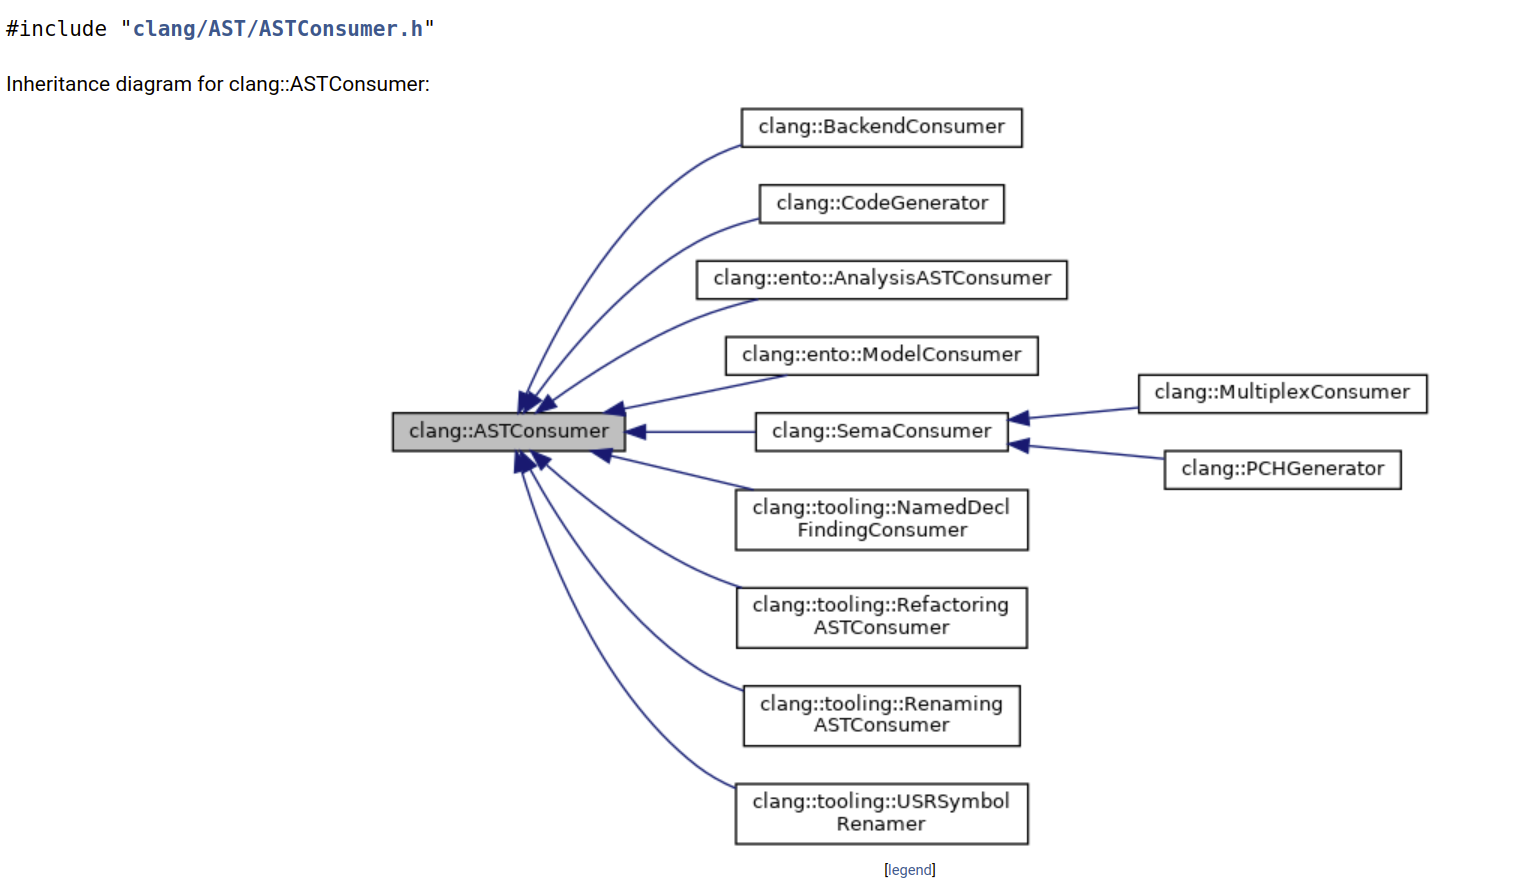
\includegraphics[scale=0.3]{ASTConsumer2.png}
\end{center}
\caption{Klase koje implementiraju \textit{ASTConsumer} interfejs}
\label{fig:exploded}
\end{figure}

Ovaj interfejs koristan je i za kreiranje samostalnih alata za stati\v{c}ku analizu koji se baziraju na analizi AST-a. U ovu svrhu mo\v{z}e se koristiti kombinacija
ovog interfejsa sa interfejsima za obilazak AST-a kao \v{s}to su AST posetioci i AST upariva\v{c}i. Klasa koja implementira neku analizu nad AST-om treba sadr\v{z}ati jedan ili vi\v{s}e objekata klasa za obilazak AST-a i zatim izvr\v{s}iti taj obilazak predefinisanjem metoda \texttt{virtual void  HandleTranslationUnit(ASTContext \&Ctx)} koji se poziva nakon \v{s}to je kreiran AST za jedinicu prevođenja. Logika same analize AST-a tokom obilaska treba biti implementirana u okviru klase koja implementira obilazak, odnosno u AST upariva\v{c}ima ili posetiocima \cite{ASTConsumer}.

\begin{lstlisting}[style=customc, caption={Primer upotrebe klase \textit{ASTConsumer} \cite{ASTToolTutorial}}, label=lst:label7, captionpos=b]
class FindNamedClassVisitor
  : public RecursiveASTVisitor<FindNamedClassVisitor> {
public:
  bool VisitCXXRecordDecl(CXXRecordDecl *Declaration) {
    Declaration->dump();
    return true;
  }
};

class FindNamedClassConsumer : public clang::ASTConsumer {
public:
  virtual void HandleTranslationUnit(clang::ASTContext &Context) {
    Visitor.TraverseDecl(Context.getTranslationUnitDecl());
  }
private:
  FindNamedClassVisitor Visitor;
};
\end{lstlisting}

\subsection{Intefejs FrontendAction}

\texttt{FrontendAction} je apstraktna klasa za akcije koje mogu biti izvr\v{s}ene od strane prednjeg dela kompajlera (eng. \textit{frontend}).
Ovu klasu karakteri\v{s}e jednostavan javni interfejs koji se sastoji od slede\'{c}ih metoda:

\begin{itemize}
  \item \texttt{bool PrepareToExecute (CompilerInstance \&CI)} \\
  Ova metoda slu\v{z}i za pripremanje primarne akcije koja \'{c}e biti izvr\v{s}ena nad objektom klase \texttt{CompilerInstance}.
  Priprema uklju\v{c}uje izmene po\v{c}etne konfiguracije kompajlera kako bi olak\v{s}ala izvr\v{s}avanje akcije.
  \item \texttt{bool BeginSourceFile (CompilerInstance \&CI, const FrontendInputFile \&Input)} \\
  Prirprema akciju za procesiranje ulaznog fajla. Ukoliko ova metoda vrati vrednost \texttt{false}, kompilacija fajla \texttt{Input} \'{c}e biti prekinuta
  i primarna akcija se ne\'{c}e izvr\v{s}iti.
  \item \texttt{llvm::Error Execute ()} \\
  Metoda odgovorna za izvr\v{s}avanje akcije. Ova metoda interno poziva \v{c}istu virtuelnu metodu \texttt{virtual void ExecuteAction()=0}
  koju svaka podklasa klase \texttt{FrontendAction} predefini\v{s}e implementiraju\'{c}i u okviru nje akciju koja \'ce biti izvr\v{s}ena.
  \item \texttt{virtual void EndSourceFile()} \\ 
  Izvr\v{s}ava post-procesiranje nakon svakog fajla, dealocira objekte, obrađuje statistiku i sređuje k\^{o}d  u izlaznom fajlu.
\end{itemize}

Klasa \texttt{FrontendAction} ima raznolike upotrebe, odnosno specijalizacije. Primer specijalizacija ove klase su \texttt{DumpCompilerOptionsAction}
koja omogu\'{c}ava ispisivanje opcija koje se mogu zadati kompajleru i \texttt{PreprocessorFrontendAction} koja omogu\'{c}ava izvr\v{s}avanje akcija vezanih za pretprocesiranje izvornog koda. Međutim, naj\v{c}es\'{c}a upotreba ovog interfejsa vezana je za akcije koje se izvr\v{s}avaju nad AST-om. U ovu svrhu koristi se apstarktna klasa \texttt{ASTFrontendAction} koja je direktna potklasa klase \texttt{FrontendAction}. \par
Ova klasa oslanja se na kori\v{s}\'{c}enje interfejsa \texttt{ASTConsumer}. Dovoljno je inicijalizovati klasu \texttt{ASTFrontendAction} objektom implementiranog \texttt{ASTConsumer}-a, a zatim u metodi \texttt{ExecuteAction()} kreirati parserom AST,
tokom \v{c}ega \'{c}e se izvr\v{s}avati akcije opisane u \texttt{ASTConsumer}-u. Neke od bitnih implementacija ovog interfejsa predstavljaju klase \texttt{CodeGenAction}, \texttt{ASTDumpAction}, \texttt{FixitAction} \cite{FrontendAction}...  Na listingu \ref{lst:label8} prikazan je primer upotrebe ovog interfejsa. 
\\
\begin{lstlisting}[style=customc, caption={Primer upotrebe klase \texttt{ASTFrontendAction} interfejsa \cite{ASTToolTutorial}}, label=lst:label8, captionpos=b]
class FindNamedClassAction : public clang::ASTFrontendAction {
public:
  virtual std::unique_ptr<clang::ASTConsumer> CreateASTConsumer(
    clang::CompilerInstance &Compiler, llvm::StringRef InFile) {
    return std::make_unique<FindNamedClassConsumer>(&Compiler.getASTContext());
  }
};

\end{lstlisting}


\begin{figure}[h!]
\begin{center}
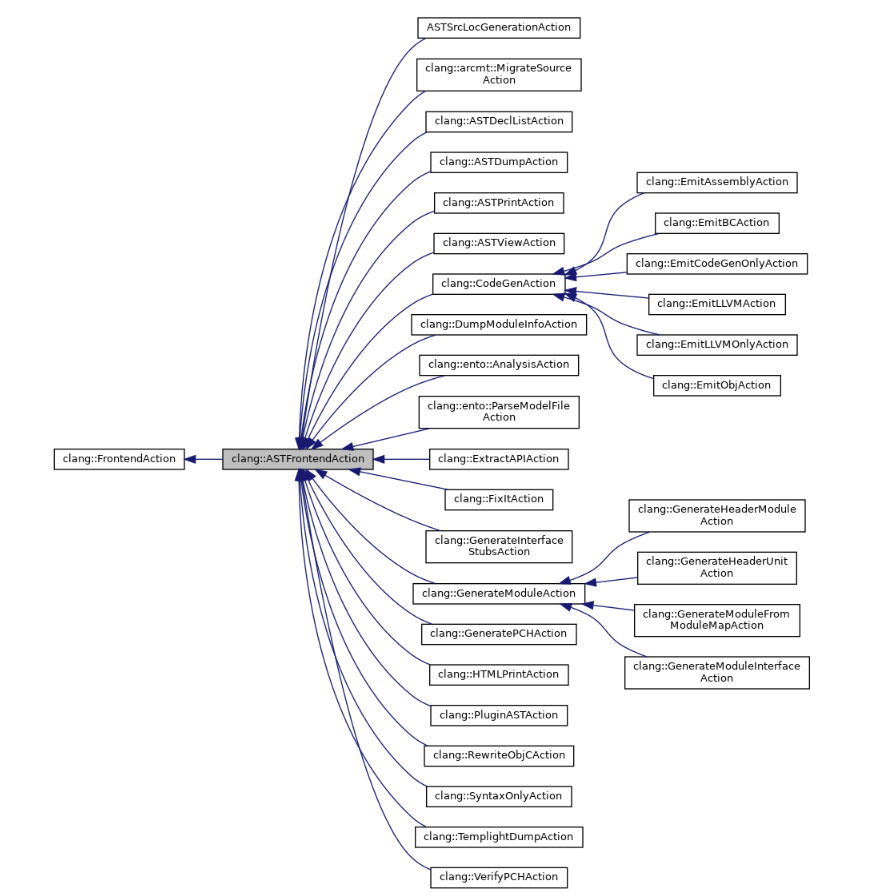
\includegraphics[scale=0.4]{ASTFrontendAction.png}
\end{center}
\caption{Klase koje implementiraju \textit{ASTFrontendAction} interfejs}
\label{fig:exploded}
\end{figure}



\section{Biblioteke za kreiranje alata}

 Kompajler Clang pru\v{z}a infrastrukturu za pisanje razli\v{c}itih softverskih alata koji koriste sintaksne i semanti\v{c}ke informacije o programu. U nastavku \'{c}e biti opisano nekoliko bibloteka koje se mogu koristiti u ovu svrhu zajedno sa njihovim prednostima i manama.


\begin{itemize}
\item \texttt{LibClang} je stabilni C interfejs ka Clang-u visokog nivoa (eng. \textit{high level}). Ovaj interfejs pru\v{z}a parsiranje izvornog koda
i izagradnju AST-a, u\v{c}itavanje ve\'{c} kreiranog AST-a, obilazak AST-a i dohvatanje određenih informacija o izgrađenom AST-u kao \v{s}to su lokacije iz izvornog koda elemenata iz stabla. Ovaj interfejs ne pru\v{z}a sve informacije i detalje iz izgrađenog AST-a \cite{LibClang}. Ovo ga \v{c}ini nepogodnim za implementaciju alata za stati\v{c}ku analizu ali omogu\'{c}ava stabilnost pri promeni verzija Clang-a.
Treba ga koristiti u slu\v{c}ajevima kada:
\begin{itemize}
  \item je potreban interfejs ka Clang-u iz jezika koji nije C++.
  \item je potreban stabilni inferfejs koji je kompatibilan sa starijim verzijama Clang-a.
  \item su potrebne apstrakcije visokog nivoa kao \v{s}to je iteriranje kroz AST sa kursorima i drugi detaljni vezani za Clang-ov AST.
\end{itemize}
LibClang ne treba koristiti kada je potrebna puna kontrola nas AST-om \cite{RightInterface}.

\item \texttt{Clang Plugins} biblioteka omogu\'{c}ava izvr\v{s}avanje dodatnih akcija nad AST-om tokom kompilacije programa. Ovo su dinami\v{c}ke biblioteke koje kompajler u\v{c}itava tokom izvr\v{s}avanja i lako ih je integrisati u okru\v{z}enje za prevođenje programa (eng. \textit{build enviroment}).

Treba ih koristiti kada:

\begin{itemize}
\item je potrebno ponovno izvr\v{s}avanje alata uvek kada se zavisnosti potrebne za prevođenje programa izmene.
\item je potrebno da alat omogu\'{c}i ili neomogu\'{c}i prevođenje programa.
\item je potrebna potpuna kontrola nad Clang-ovim AST-om.
\end{itemize}
Ne treba ih koristiti kada:
\begin{itemize}
\item je potrebno kreirati alat koji se ne koristi u okviru sistema za prevođenje programa.
\item su alatu potrebne informacije o tome kako je Clang pode\v{s}en uklju\v{c}uju\'{c}i mapiranje virtuelnih fajlova u memoriji.
\item je potrebno koristiti alat nad podskupom fajlova u projektu koji nisu povezani sa izmenama koje bi zahtevale ponovno prevođenje programa \cite{RightInterface}.
\end{itemize}

\item \texttt{LibTooling} je C++ interfejs koji slu\v{z}i za pisanje samostalnih alata. Ova biblioteka omogu\'{c}ava jednostavnu
upotrebu opisanih akcija prednjeg dela kompajlera (eng. frontend actions), ali i jednostavno dodavanje opcija komandne linije i pokretanje nad fajlovima 
nezavisnim od sistema za prevođenje. Ova svojstva \v{c}ine \texttt{LibTooling} biblioteku najkorisnijom od prethodno opisanih bibloteka u svrhu kreiranja alata za stati\v{c}ku analizu.
Uopsteno, \texttt{LibTooling} treba koristiti kada:
\begin{itemize}
  \item je potrebno pokretati alat nad jednim fajlom ili specifi\v{c}nim podskupom fajlova nezavisnim od sistema za prevođenje.
  \item je potrebno imati punu kontrolu nad Clang-ovim AST-om.
  \item je potrebno deliti k\^{o}d  sa Clang-ovim Plugin-ovima.
\end{itemize}
\texttt{LibTooling} nije najbolji izbor u slu\v{c}ajevima kada:
\begin{itemize}
  \item je potrebno pokretati alat nakon promena u zavisnostima u sistemu za prevođenje.
  \item je potreban stabilan interfejs tako da se k\^{o}d  alata ne mora menjati kada se AST API (eng. \textit{Application Programming Interface}) promeni.
  \item su potrebne apstrakcije visokog nivoa kao \v{s}to su kursori.
  \item alat ne\'{c}e biti napisan u C++-u \cite{RightInterface}.
\end{itemize}
\end{itemize}

Na listingu \ref{lst:label9} prikazana je implementacija jednostavnog alata kori\v{s}\'{c}enjem opisanih interfejsa \texttt{ASTVisitor}, \texttt{ASTConsumer} i \texttt{FrontendAction}. Ovaj alat koristi \texttt{libtooling} biblioteku za pokretanje definisane \texttt{FrontendAction} akcije nad izvornim kodom koji je prosleđen kao argument komandne linije. Alat ispisuje lokacije svih struktura, unija i klasa sa imenom \texttt{n::m::C}. 
\\
\begin{lstlisting}[style=customc, caption={Primer implementacije jednostavnog alata upotrebom interfejsa \texttt{ASTVisitor}, \texttt{ASTConsumer}, \texttt{FrontendAction} i bibliotekom \texttt{libtooling} \cite{ASTToolTutorial}}, label=lst:label9, captionpos=b]
#include "clang/AST/ASTConsumer.h"
#include "clang/AST/RecursiveASTVisitor.h"
#include "clang/Frontend/CompilerInstance.h"
#include "clang/Frontend/FrontendAction.h"
#include "clang/Tooling/Tooling.h"

using namespace clang;

class FindNamedClassVisitor
  : public RecursiveASTVisitor<FindNamedClassVisitor> {
public:
  explicit FindNamedClassVisitor(ASTContext *Context)
    : Context(Context) {}

  bool VisitCXXRecordDecl(CXXRecordDecl *Declaration) {
    if (Declaration->getQualifiedNameAsString() == "n::m::C") {
      FullSourceLoc FullLocation = Context->getFullLoc(Declaration->getBeginLoc());
      if (FullLocation.isValid())
        llvm::outs() << "Found declaration at "
                     << FullLocation.getSpellingLineNumber() << ":"
                     << FullLocation.getSpellingColumnNumber() << "\n";
    }
    return true;
  }

private:
  ASTContext *Context;
};

class FindNamedClassConsumer : public clang::ASTConsumer {
public:
  explicit FindNamedClassConsumer(ASTContext *Context)
    : Visitor(Context) {}

  virtual void HandleTranslationUnit(clang::ASTContext &Context) {
    Visitor.TraverseDecl(Context.getTranslationUnitDecl());
  }
private:
  FindNamedClassVisitor Visitor;
};

class FindNamedClassAction : public clang::ASTFrontendAction {
public:
  virtual std::unique_ptr<clang::ASTConsumer> CreateASTConsumer(
    clang::CompilerInstance &Compiler, llvm::StringRef InFile) {
    return std::make_unique<FindNamedClassConsumer>(&Compiler.getASTContext());
  }
};

int main(int argc, char **argv) {
  if (argc > 1) {
    clang::tooling::runToolOnCode(std::make_unique<FindNamedClassAction>(), argv[1]);
  }
}

\end{lstlisting}


\chapter{Alat Autofix}
\label{chp:autofix}

Alat \textit{Autofix} predstavlja alat za stati\v{c}ku analizu izvornog koda napisanog u jeziku C++14. Alat prijavljuje upozorenja
za kod koji nije napisan u skladu sa odabranim podskupom pravila iz standarda kodiranja \textsc{autosar c++14} i zajedno sa upozorenjima
ispisuje predlog k\^{o}da kojim se po\v{c}etni k\^{o}d mo\v{z}e zameniti kako bi bio u skladu sa standardom.
Alat je implementiran u programskom jeziku \textit{C++} kori\v{s}\'{c}enjem biblioteka za razvoj alata dostupnim u okviru kompajlerske infrastrukture LLVM.
Osnovna svrha alata je demonstracija kreiranja alata u okviru kompajlerske infrastrukture LLVM i predstavljanje tehnika obilaska i analize Clang-ovog AST-a. 
Alat je dostupan i nalazi se na linku \url{https://github.com/ognjen-plavsic/master/tree/main/code}. Na pomenutom linku se nalaze neophodne datoteke alata, opis
sistema, kao i skup test primera i njihova pokretanja.

\section{Kori\v{s}\'{c}enje alata}

Alat \textit{Autofix} se pokre\'{c}e komandom:
\\ \\
 \indent \indent \texttt{auto-fix [options] <source0> [... <sourceN>]}
\\ 

Navedeni arumenti podrazumevaju sledeće:
\begin{itemize}
  \item \textbf{options} - Ovde spadaju opcije koje se mogu proslediti alatu \textit{Autofix}. Podr\v{z}ane su opcije:
  \begin{enumerate}
    \item \textbf{--apply-fix}: Ovom opcijom se predlo\v{z}ene izmene mogu primeniti na kod, menjaju\'{c}i izvorni fajl nad kojim je pokrenuta analiza.
    Predlozene izmene bi\'{c}e primenjene na kod ukoliko među njima ne postoji konflikt, odnosno ukoliko se razli\v{c}iti predlozi ne odnose na isti deo koda.
    \item \textbf{--list-rules}: Ispisuje sva podr\v{z}ana pravila u okviru alata u formatu \texttt{oznaka: tekst-pravila} gde je \texttt{oznaka} jedinstvena oznaka pravila iz \textsc{autosar} dokumenta, a \texttt{tekst-pravila} prestavlja kratak opis pravila iz \textsc{autosar} dokumenta koji se ujedno ispisuje prilikom prijavljivanja upozorenja vezanih za to pravilo. Primer: \\ \\
  \texttt{A7-1-8 - A non-type specifier shall be placed before a type specifier in a declaration.} \\
    \item \textbf{--rules=<string>}: Omogu\'{c}ava navođenje podskupa implementiranih pravila za koje ce alat izvr\v{s}iti analizu. Pravila u okviru ove opcije
    se navode po svojoj oznaci iz \textsc{autosar} dokumenta i treba ih razdvojiti zarezom. Ukoliko se umesto opcije pravila prosledi string \textit{all} alat \'{c}e pokrenuti
    analizu sa svim implementiranim pravilima u okviru alata. Primer kori\v{s}\'{c}enja ove opcije: \newline\newline
    \texttt{bin/auto-fix ./AutoFixTest.cpp -rules="A7\_2\_3, A7\_1\_6"} \\
    \item \textbf{--help}: Ispisuje uputstvo za upotrebu alata.
  \end{enumerate}

\item \textbf{<source0> [... <sourceN>]} - Predstavlja listu fajlova, razdvojenih razmakom, nad kojima \'{c}e se pokrenuti alat.

\end{itemize}

\section{Opis implementiranih pravila}

Pored formalne klasifikacije, pravila u okviru samog dokumenta standarda \textsc{autosar} C++14  kodiranja struktuirana su po poglavljima.
Struktura poglavlja ovog dokumenta slična je strukturi iz samog C++ standarda ISO/IEC 14882:2014. Svako poglavlje odgovara jednoj komponenti (svojstvu) C++14 jezika, to jest, sadrži pravila koja se odnose na tu komponentu.
\\
\indent
Pravila razmatrana u ovom radu predstavljaju podskup pravila koja se odnose na deklaracije. Razlog za ovo je dvojak. Deklaracije predstavljaju jedan
od osnovnih i najvažnijih koncepta u C++-u i programiranju generalno. U C++-u deklaracije čine samu srž ekspresivne moći jezika i u direktnoj su vezi
sa naprednijim konceptima jezika i računarastva, kao što je, na primer, šablonsko metaprogramiranje (\textit{eng. template metaprogramming}).
Sa druge strane jednostavnost sintakse deklaracija u C++-u čini pogodno tlo za korišćenje kompajlerskih tehnika i struktura u okviru kompajlera Clang kojim se mogu analizirati konstrukti jezika koji nisu u skladu sa pravilima i predlagati prikladne alternative.
\\
\indent
Sva implementirana pravila u okviru projekta spadaju, prema klasifikaciji iz prethodnog poglavlja, u sledeće kategorije:
\begin{enumerate}
  \item{Obavezna, prema klasifikaciji po obavezi.}
  \item{Automatizovana, prema klasifikaciji po primenjivosti statičke analize.}
  \item{Implementaciona, prema klasifikaciji po cilju primene.}
\end{enumerate}

Razmatrana pravila nisu nužno implementirana u potpunosti u okviru alata Autofix, iako činjenica da pravila spadaju u kategorije obaveznih i automatizovanih
implicira da je to teorijski moguće uraditi. Pravila koje Autofix podržava birana su tako da se ograničenja koja potiču iz same prirode projekta minimalno manifestuju. Ograničenja potiču od primarnih tehnologija i biblioteka kojima je alat implementiran ali i činjenice da se alat zasniva na predlogu izmena koda. 
stati\v{c}ki analizator kompajlera Clang \cite{CSAWebsite} (eng. \textit{Clang Static Analyzer}) nije korišćen u okviru ovog alata, tako da su pravila izabrana tako da što manji broj slučajeva upotrebe zahteva simboličko izvršavanje programa. Drugo ograničenje potiče iz činjenice da u nekim slučajevima nije moguće ili je znatno komplikovanije kreirati predlog ispravke koda (\textit{eng. fixit hint}). Pravila razmatrana u okviru ovog rada birana su tako da se većina konstrukta koji nisu u saglasnosti sa pravilom mogu detektovati analizom Clang-ovog AST-a i da se za njih mogu kreirati razumne alternative koje su u skladu sa standardom \textsc{autosar} C++14.

\section{Primeri rada alata}

U ovoj sekciji bi\'{c}e navedena sva pravila iz \textsc{autosar} dokumenta koje alat \textit{Autofix} podr\v{z}ava i bi\'{c}e prikazani primeri rada alata za svako od tih pravila.
Primeri \'{c}e sadr\v{z}ati izvorni kod programa nad kojim se alat pokre\'{c}e i ispis na standardnom izlazu koji predstavlja rezultat izvr\v{s}avanja alata. U primeru rada alata
pri zadavanju opcije \texttt{--apply-fix} bi\'{c}e prikazan i kod nakon zavr\v{s}etka rada alata, odnosno kod za primenjim predlozima izmena.\\

\begin{primer}
         Pravilo A7-1-8 (obvezno, implementaciono, automatizovano) \newline
         U deklaracijama specifikatori koji nisu vezani za tipove treba da stoje
         ispred tipskih specifikatora.
\end{primer}

Razmotrimo kod sa listinga \ref{lst:label12}. Deklaracija metoda \texttt{f3} sadr\v{z}i tri specifikatora: \texttt{void}, \texttt{virtual} i \texttt{inline}.
Specifikator \texttt{void} ozna\v{c}ava "prazan" tip, odnosno da metoda \texttt{f3} nema povratnu vrednost. Stoga, \texttt{void} spada u tipske specifikatore.
Specifikator \texttt{virtual} omogu\'{c}ava dinami\v{c}ki polimorfizam dok \texttt{inline} predla\v{z}e kompajleru da kod ove funkcije umetne u funkciju iz koje je pozvana
kako bi se izbeglo dodatno vreme potrebno za pozivanje funkcije. Dakle \texttt{virtual} i \texttt{inline} se ne odnose na tipove i nisu tipski specifikatori. Pravilo
\texttt{A7-1-8} nala\v{z}e da se specifikator \texttt{void} u deklaraciji nađe nakon specifikatora \texttt{virtual} i  \texttt{inline}, odnosno da metod \texttt{f3} bude
deklarisan kao metod \texttt{f1} ili metod \texttt{f2}. sli\v{c}no va\v{z}i i za deklaraciju promenljive \texttt{x} i specifikatore \texttt{std::int32\_t} i \texttt{mutable}. \\ 


\begin{lstlisting}[style=customc, caption={Primer koda koji nije napisan u skladu sa pravilom A7-1-8}, label=lst:label12, captionpos=b]
#include <cstdint>

class C {
public:
  virtual inline void f1();
  inline virtual void f2();
  void virtual inline f3();

private:
  std::int32_t mutable x;
  mutable std::int32_t y;
};
\end{lstlisting}

\begin{figure}[!h]
\begin{center}
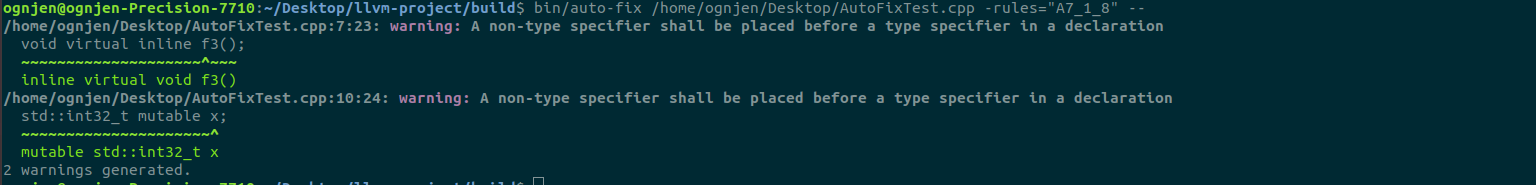
\includegraphics[scale=0.3]{A7-1-8.png}
\end{center}
\caption{Ispis alata za pravilo A7-1-8}
\label{fig:A7-1-8}
\end{figure}

\begin{primer}
Pravilo A8-5-3 (obvezno, implementaciono, automatizovano) \\
Varijabla tipa \texttt{auto} ne sme biti inicijalizovana kori\v{s}\'{c}enjem
inicijalizacijom viti\v{c}astih zagrada tipa \{\} ili =\{\}.
\end{primer}

Po standardu C++14 kompajler \'{c}e \texttt{auto} promenljivu inicijalizovanu sinaksom viti\v{c}astih zagrada tretirati kao objekat klase
\texttt{std::initializer\_list}. Međutim neki kompajleri mogu implementirati ovo druga\v{c}ije i zaklju\v{c}iti tip \texttt{int} za objekat inicijalizovan
sintaksom \texttt{\{\}}, dok \'{c}e za sintaksu \texttt{=\{\}} zaklju\v{c}iti tip \texttt{std::initializer\_list}. Da bi se izbegla konfuzija oko zaklju\v{c}ivanja
tipova, \textsc{autosar} standard nala\v{z}e da se ne koristi nijedna od navede dve vrste inicijalizacije. Za kod sa listinga \ref{lst:label13} \textit{Autofix} \'{c}e
predlo\v{z}iti inicijalizaciju simbolom \texttt{=}. Ispis alata prikazan je na slici \ref{fig:A8-5-3}. \\

\begin{lstlisting}[style=customc, caption={Primer koda koji nije napisan u skladu sa pravilom A8-5-3}, label=lst:label13, captionpos=b]
#include <initializer_list>

void fn() noexcept {
  auto x1(10);
  auto x2{10};
  auto x3 = 10;
  auto x4 = {10};
}

\end{lstlisting}

\begin{figure}[!h]
\begin{center}
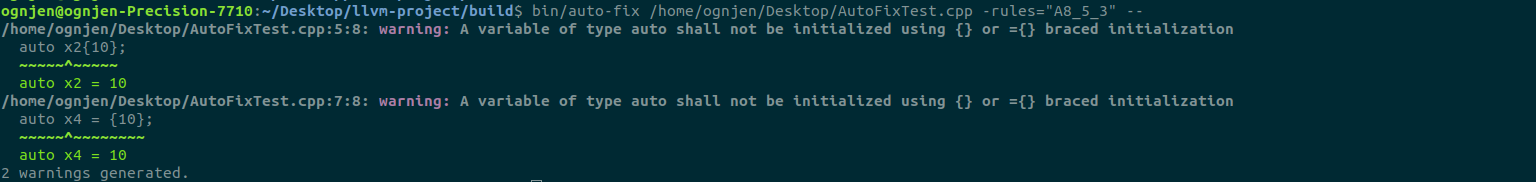
\includegraphics[scale=0.3]{A8-5-3.png}
\end{center}
\caption{Ispis alata za pravilo A8-5-3}
\label{fig:A8-5-3}
\end{figure}

\begin{primer}
Pravilo A8-5-2 (obvezno, implementaciono, automatizovano) \\
Inicijalizacija viti\v{c}astim zagradama bez znaka jednako (\texttt{=}) treba biti kori\v{s}\'{c}ena za inicijalizaciju promenljive.
\end{primer}

\textsc{autosar} zahteva upotrebu ove inicijalizacije kako bise izbegla dvosmislenost u kodu. Na primer, upotreba znaka jednako (\texttt{=}) pri
inicijalizaciji navodi programere na pomisao da dolazi do dodeljivanja vrednosti iako se zapravo vr\v{s}i kreiranje i inicijalizacija objekta.
Takođe ukoliko se koristi predo\v{z}ena sintaksa ne\'{c}e do\'{c}i do konverzija tipova iz tipa ve\'{c}e bitske \v{s}irine u tip manje bitske \v{s}irine (eng. \textit{narrowing conversions}),
\v{s}to je ujedno \v{c}ini i sigurnijom od ostalih vrsta inicijalizacija. Ispis alata pokrenutim nad fajlom sa kodom iz listinga \ref{lst:label14} prikazan je na slici \ref{fig:A8-5-2}. \\

\begin{lstlisting}[style=customc, caption={Primer koda koji nije napisan u skladu sa pravilom A8-5-2}, label=lst:label14, captionpos=b]
#include <cstdint>
#include <initializer_list>

void f1() noexcept {
  std::int32_t x1 = 8;
  std::int8_t x2{50};
  std::int8_t x3 = {50};
  std::int8_t x4 = 1.0;
  std::int8_t x5 = 300;
  std::int8_t x6(x5);
}
\end{lstlisting}

\begin{figure}[!h]
\begin{center}
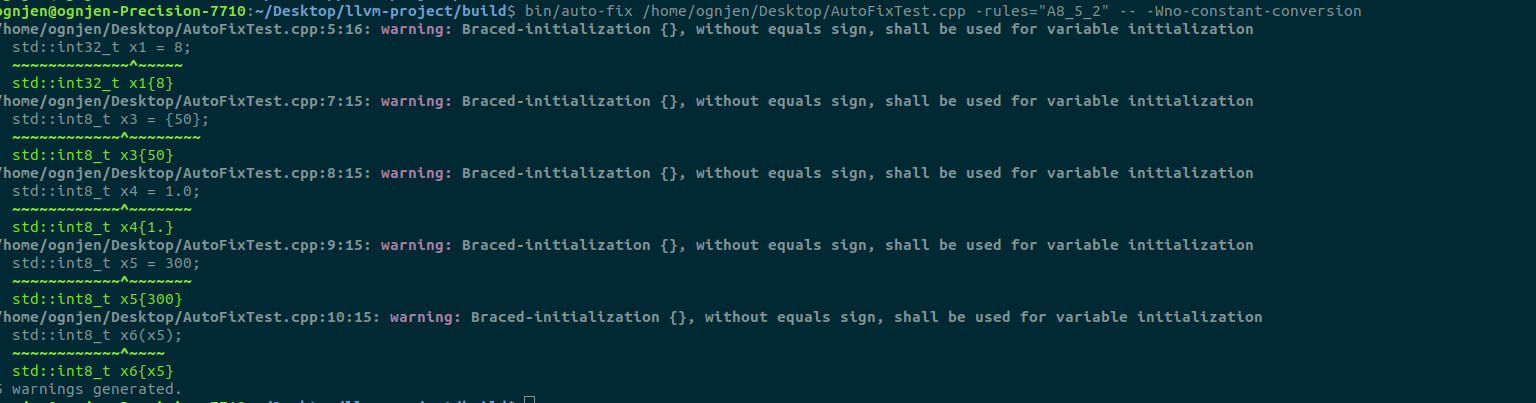
\includegraphics[scale=0.3]{A8-5-2.png}
\end{center}
\caption{Ispis alata za pravilo A8-5-2}
\label{fig:A8-5-2}
\end{figure}

\begin{primer}
Pravilo A7-1-6 (obvezno, implementaciono, automatizovano) \\
Ne treba koristiti specifikator \texttt{typedef}. 
\end{primer}

Specifikator \texttt{typedef} nije pogodan za kreiranje pseudionima (eng. \textit{alias}) za \v{s}ablonske tipove ali i \v{c}ini kod manje \v{c}itljivim.
Oba nedostatka mogu se zaobi\'{c}i kori\v{s}\'{c}enjem specifikatora \texttt{using}. Alat \textit{Autofix} od izraza za kreiranje pseudonima za tip kori\v{s}\'{c}enjem
specifikatora \texttt{typedef} kreira i ispisuje analogni izraz koji koristi \texttt{using} sintaksu. Ispis alata pokrenutim nad fajlom sa kodom iz listinga \ref{lst:label15} prikazan je na slici \ref{fig:A7-1-6}. \\

\begin{lstlisting}[style=customc, caption={Primer koda koji nije napisan u skladu sa pravilom A7-1-6}, label=lst:label15, captionpos=b]
#include <cstdint>

typedef unsigned long ulong;
typedef std::int32_t (*fPointer1)(std::int32_t);
typedef int int_t, *intp_t;

\end{lstlisting}

\begin{figure}[!h]
\begin{center}
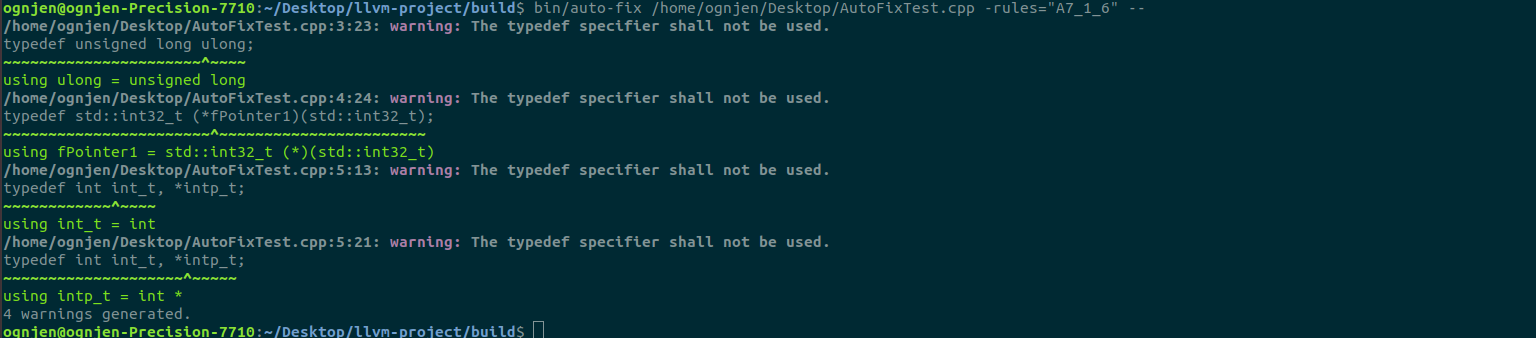
\includegraphics[scale=0.3]{A7-1-6.png}
\end{center}
\caption{Ispis alata za pravilo A7-1-6}
\label{fig:A7-1-6}
\end{figure}


\begin{primer}
Pravilo A7-2-3 (obvezno, implementaciono, automatizovano) \\
Nabrajanja (eng. \textit{enumerators}) treba deklarisati kao nabrajanja sa opsegom odnosno treba koristiti \texttt{scoped enum class} sintaksu.
\end{primer}

Ukoliko je nabrajanje bez opsega deklarisano u globalnom opsegu, onda njegove vrednosti mogu ponovo deklarisati konstante koje su deklarisane sa istim identifikatorom u globalnom opsegu. Kori\v{s}\'{c}enjem nabrajanja sa opsegom, odnosno upotrebom \texttt{scoped enum class} sintakse, identifikatori kori\v{s}\'{c}eni prilikom
nabrajanja bi\'{c}e deklarisani u svom unutra\v{s}njem opsegu i time spre\v{c}iti ponovno deklarisanje identifikatora iz spolja\v{s}njeg opsega. 
Ispis alata \textit{Autofix} pokrenutim nad fajlom sa kodom iz listinga \ref{lst:label16} prikazan je na slici \ref{fig:A7-2-3}. \\

\begin{lstlisting}[style=customc, caption={Primer koda koji nije napisan u skladu sa pravilom A7-2-3}, label=lst:label16, captionpos=b]
#include <cstdint>

enum E1 : std::int32_t { E10, E11, E12 };

\end{lstlisting}


\begin{figure}[!h]
\begin{center}
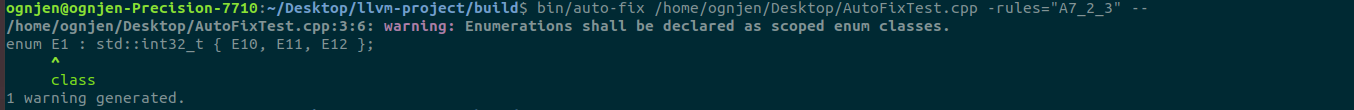
\includegraphics[scale=0.3]{A7-2-3.png}
\end{center}
\caption{Ispis alata za pravilo A7-2-3}
\label{fig:A7-2-3}
\end{figure}
% ------------------------------------------------------------------------------

% \pangrami

% \pangrami

% ------------------------------------------------------------------------------
\chapter{Zaključak}
% ------------------------------------------------------------------------------
% \pangrami

% \pangrami

% ------------------------------------------------------------------------------
% Literatura
% ------------------------------------------------------------------------------
\literatura

% ==============================================================================
% Završni deo teze i prilozi
\backmatter
% ==============================================================================

% ------------------------------------------------------------------------------
% Biografija kandidata
\begin{biografija}
  % \textbf{Ognjen Plavšić} (\emph{Tršić,
  %   26. oktobar/6. novembar 1787. — Beč, 7. februar 1864.}) bio je
  % srpski filolog, reformator srpskog jezika, sakupljač narodnih
  % umotvorina i pisac prvog rečnika srpskog jezika.  Vuk je
  % najznačajnija ličnost srpske književnosti prve polovine XIX
  % veka. Stekao je i nekoliko počasnih mastera.  Učestvovao je u
  % Prvom srpskom ustanku kao pisar i činovnik u Negotinskoj krajini, a
  % nakon sloma ustanka preselio se u Beč, 1813. godine. Tu je upoznao
  % Jerneja Kopitara, cenzora slovenskih knjiga, na čiji je podsticaj
  % krenuo u prikupljanje srpskih narodnih pesama, reformu ćirilice i
  % borbu za uvođenje narodnog jezika u srpsku književnost. Vukovim
  % reformama u srpski jezik je uveden fonetski pravopis, a srpski jezik
  % je potisnuo slavenosrpski jezik koji je u to vreme bio jezik
  % obrazovanih ljudi. Tako se kao najvažnije godine Vukove reforme
  % ističu 1818., 1836., 1839., 1847. i 1852.
\end{biografija}
% ------------------------------------------------------------------------------

\end{document}
